
\documentclass[12pt]{article}

\usepackage{sbc-template}
\usepackage[square,authoryear]{natbib}
\usepackage{graphicx,url}   
%\usepackage[latin1]{inputenc}  
\usepackage[brazil]{babel} 
\usepackage[utf8]{inputenc}      
%\usepackage{placeins}
%\usepackage[monochrome]{color}
\usepackage{verbatim} %para inserir comentarios
\usepackage{todonotes}  
\usepackage{array}
%\usepackage{pgfplots}
%\pgfplotsset{width=.8\textwidth}
%\usepgfplotslibrary{external}
%\tikzexternalize



\sloppy

\title{Uma proposta de metodologia de pesquisa de patentes verdes utilizando padrões frequentes}

\author{}
\address{CEFET/RJ - Centro Federal de Educação Tecnológica Celso Suckow da Fonseca\\
  Av. Maracanã, 229 - Rio de Janeiro - RJ - Brasil. \\
  \\
\begin{minipage}{1\textwidth}
\begin{flushleft}
%Orientadores escolhidos: Jorge de Abreu Soares, Eduardo Ogasawara, Gustavo Guedes.\\
%Linha de pesquisa: Gerência de Dados e Aplicações\\
%Projeto de pesquisa: Mineração de Dados e Aprendizado de Máquina\\
\end{flushleft}
\end{minipage}
}

\begin{document}

\maketitle


\begin{abstract}
With technological innovations advancement, a large number of documents are being generated in the form of patent registrations. Thus, the need for new techniques and tools capable of organizing and analyzing this data to present them with satisfactory performance increases. This paper aims to present a new approach to patent research and to make comparisons with methods studied today. Specifically, it conducts a study using a subset of patents called ``green patents'', developing a methodology for researching green patents using frequent pattern mining. We also present the expected contributions to the end of this work.

\end{abstract}


\begin{resumo} 

Com o avanço das inovações tecnológicas, vem sendo gerada uma grande quantidade de documentos na forma de registros de patentes. Desta forma, cresce a necessidade de se obter novas técnicas e ferramentas capazes de organizar e analizar esses dados para apresentá-los com uma performance satisfatória. Este trabalho tem por objetivo apresentar uma nova abordagem de pesquisa de patentes e realizar comparações com métodos estudados nos dias de hoje. Especificamente, realiza um estudo utilizando um subconjunto de patentes denominado ``patentes verdes'', desenvolvendo uma metodologia para pesquisa de patentes verdes utilizando mineração de padrões frequentes. Também são apresentadas as contribuições esperadas ao fim deste trabalho. 

\end{resumo}

\section{Introdução}
\label{sec:intro}

O registro de patentes serve como um indicador de atividades econômicas e tecnológicas, motivando o desenvolvimento tecnológico e de ideias. Isso se deve pela exclusividade de lucro que um inventor passa a ter como direito pelo registro de suas invenções \citep{ernst2003patent, almeida1997exploration}. Questões de competitividade, inovação e custos contribuem como estímulo às empresas em desenvolverem tecnologia e registrar novas patentes, o que vem resultando num grande aumento da quantidade de registro de patentes, necessitando sistemas eficazes e eficientes para administrar essa grande quantidade de dados \citep{shalaby2017patent}. 

Além dessas questões, outros fatores acabam por influenciar um aumento desse desenvolvimento de tecnologias em áreas específicas. 
Tratados internacionais sobre meio ambiente vêm causando pressões regulatórias e normativas sobre questões ambientais, o que acaba por influenciar positivamente empresas a buscarem soluções que causem menor impacto ambiental \citep{berrone2013necessity}.
Um notório exemplo disso é a política de transição energética da Alemanha (\textit{Energiewende}), que foi responsável por mais que triplicar o número absoluto de patentes alemãs de energia eólica entre $2005$ e $2010$, aumentando em um quarto o número de patentes de energia solar fotovoltaica no mesmo período \citep{pegels2014germany}.

Com os volumes cada vez maiores de informações de patentes, as tarefas de busca e análise de patentes tornaram-se vitais sob perspectivas legais e gerenciais \citep{liu2011development}.
Isso mostra importância de metodologias e ferramentas desenvolvidas para analizar dados de patentes e apresentá-los com uma performance satisfatória, tais como \textit{Patent retrieval}.

\textit{Patent retrieval} é considerado uma ferramenta fundamental para a maioria das tarefas de analise de patentes. Seu desenvolvimento foi motivado por alguns problemas específicos ao tentar aplicar técnicas tradicionais de  mineração de texto à análise de patentes  \citep{shalaby2017patent}. 
Dentre eles, está o fato de que registros de patentes são combinações de texto descritivo \textbf{não-estruturados} (e.g., ``Título da Patente'', ``Resumo da Patente'' e a ``Descrição da Patente''), e dados bibliográficos \textbf{estruturados} relacionados a cada patente (e.g.,  ``Inventores'', ``Concessionários'' e ``Citações'') \citep{liu2011development} .

Apesar da importância do tema, ainda é uma área que carece de estudos desenvolvendo metodologias a serem empregadas na tarefa, sendo encontrados poucos trabalhos que tratam de \textit{Patent retrieval} \citep{abbas2014literature,shalaby2017patent}.
Além disso, os resultados em tarefas de \textit{Patent retrieval} apresentam desempenho mediano, mesmo nos trabalhos apontados como estado da arte \citep{shalaby2017patent}.
Considerando este cenário, essa proposta de pesquisa tem por objetivo obter melhores resultados em tarefas de \textit{Patent retrieval},  desenvolvendo para isso uma combinação de abordagens que usam conceitos de mineração de textos, associadas às técnicas de mineração de padrões frequentes.

O restante desse trabalho está organizado da seguinte forma: na Seção~\ref{sec:conceitos}, são apresentados conceitos sobre temas abordados neste estudo, de forma a falar sobre  mineração de texto, especificamente \textit{Patent retrieval}, detalhando também os conceitos de mineração de padrões frequentes. 
Na Seção~\ref{sec:met}, é descrita a metodologia proposta neste estudo.
Na Seção \ref{sec:trab}, são relacionados trabalhos referentes à analise e apresentação de dados de patentes.
Por fim, na Seção~\ref{sec:conclusao}, há uma discussão sobre as conclusões e cenários futuros.

\section{Conceitos}
\label{sec:conceitos}

\subsection{Mineração de Patentes}
\label{subsec:patmining}

Patentes são a concessão de um título de propriedade temporária de invenções de produtos, equipamentos, ferramentas e até mesmo de procedimentos e métodos de negócio \citep{mansfield1986patents}.

\cite{madani2016evolution}, existem três estágios principais da
evolução da mineração de patentes. No primeiro estágio, as metodologias mais
utilizadas eram a análise bibliométrica e a análise de citações. O segundo estágio foi
caracterizado pelo maior uso da análise de \textit{clusters} e de redes. No terceiro estágio a
mineração de patentes evoluiu para métodos de análise que utilizam a mineração de
textos e outras metodologias complementares, como análise semântica e análise
ontológica.

\cite{liu2011development} apresenta um fluxo genérico de analise de patente detalhado como pode ser observado na Figura~\ref{fig:fluxo}.

%deixa essa tambem
\begin{figure}[!h]
\centering
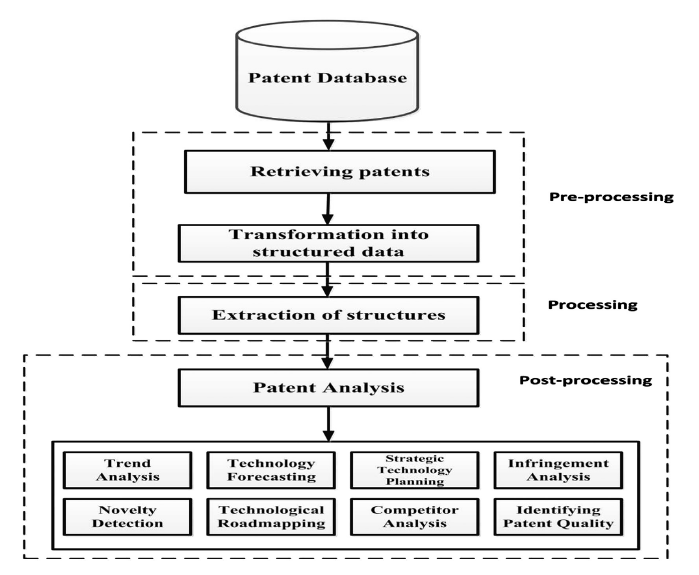
\includegraphics[width=.8\textwidth]{Workflow.PNG}
\caption{Fluxo genérico de Análise de Patente (adaptado de \cite{abbas2014literature})}
\label{fig:fluxo}
\end{figure}
%\FloatBarrier


\subsection{Mineração de Padrões Frequentes}
\label{subsec:padroes}
O processo conhecido como mineração de dados consiste em  explorar grandes quantidades de dados, de forma a extrair ou ajudar na obtenção de informações interessantes \citep{han2011data}. O uso de técnicas da área de mineração de dados vem atender a necessidade de  análise destes dados, considerando a grande quantidade de dados sendo gerados e armazenados a todo momento na atualidade \citep{chen2014big}. Essa área é focada na automatização da análise de grandes conjuntos de dados, gerando novos subconjuntos organizados de forma a encontrar padrões consistentes, destacando-se técnicas conhecidas como regras de associação, análise de sequências temporais e mineração de padrões frequentes \citep{han2011data}.

A mineração de padrões frequentes é um método para extrair conhecimento de dados buscando padrões recorrentes. Dentre diversas técnicas para mineração de padrões frequentes, pode ser utilizado o algoritmo Apriori \citep{agrawal1994fast}. Esse algoritmo busca por padrões e encontra conjuntos de itens frequentes, podendo resultar em conhecimento novo e útil sobre associações e correlações entre dados \citep{james2013introduction}.

Ao concluir a execução de técnica para mineração de padrões frequentes, apresenta-se como resultado algo na forma: ``SE  X, ENTÃO Y''. Ou seja, em uma mesma transação aparece uma representação de um ou mais elementos que levam à presença de outro elemento ou elementos (`transação' indicando, aqui, quais itens foram consultados em uma determinada operação de consulta). Com isso se encontram relacionamentos ou padrões frequentes, como conjuntos de itens frequentes, subsequencias frequentes e subestruturas frequentes, entre conjuntos de dados \citep{han2011data}. 

Padrões que refletem itens que são frequentemente associados podem ser representados sob a forma de regras de associação. Essas regras possuem medidas chamadas de suporte e confiança. O suporte representa a proporção  de transações em análise  em que os itens identificados aparecem juntos. 
Confiança representa a proporção que dado item aparece junto de outro, dentro do subconjunto em que dado item sempre aparece. As regras de associação que são consideradas interessantes são aquelas que alcançam os valores mínimos de suporte e confiança.

Porém, mesmo com a delimitação de valores mínimos para suporte e confiança, pode acontecer de ser encontrado um número enorme de regras geradas. Isso acontece principalmente quando os valores mínimos de suporte e confiança são muito baixos. Assim, é utilizada também uma medida chamada \textit{lift}  (elevação) \citep{webb2000efficient}, como forma de análise adicional para selecionar regras mais relevantes.


\section{Metodologia Proposta}
\label{sec:met}

Conforme ilustrado na Figura~\ref{fig:tratamento}, a metodologia para desenvolvimento deste trabalho se baseia, inicialmente, em analisar um conjunto de dados (``conjunto de treinamento'') e organizá-los de acordo com padrões. O reconhecimento de padrões visa classificar dados baseados em conhecimento\textit{ a priori} (i.e., preliminar ou dedutivo) ou informações estatísticas extraídas de padrões. 
Em seguida, usar matriz de similaridade e realizar uma técnica de mineração de textos (\textit{textmining}) para comparação, e então avaliar o melhor método que traz os resultados.
Replicar os métodos que são mais utilizados para gerar dados para comparação dos métodos.

\begin{figure}[!h]
\centering
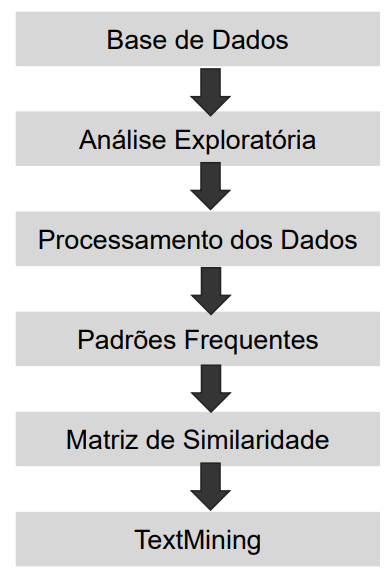
\includegraphics[width=.4\textwidth]{Metodologia_.png}
\caption{Sequência de tratamento dos dados}
\label{fig:tratamento}
\end{figure}
%\FloatBarrier


Serão aplicadas técnicas de pré-processamento, antes de se buscar por padrões frequentes nos dados de patentes obtidos. Considerando as etapas encontradas na literatura, são previstas as tarefas de integração, redução e transformação dos dados utilizados. O objetivo desta etapa é de aumentar a qualidade e o poder de expressão dos dados a serem minerados \citep{han2011data}. Em seguida, será dada sequência à busca por padrões frequentes.

Referente à metodologia utilizada para busca de padrões frequentes em dados de patentes, o processo será baseado nas atividades de geração de regras e análise de regras.  Na geração de regras é aplicado um princípio \textit{a priori} para produzir regras de associação. Podem ser atribuídos valores de suporte e a confiança de $0,01$ e $0,5$, respectivamente, como forma de limitar o número de regras obtidas. Estudos de trabalho na literatura serão buscados como subsídio para cálculo do valor utilizado, de forma a reduzir a quantidade de regras a serem interpretadas durante a análise de regras sem prejuízo para a tarefa. 

A aprendizagem de regras de associação envolve técnicas de análise destinadas a descobrir as associações e conexões entre itens específicos. Para geração de regras de regras de associação, se utiliza o algoritmo Apriori, por exemplo. Proposto em $1994$, trata-se de um algoritmo que resolve o problema da mineração de \textit{itemsets} frequentes. Ou seja, dados um banco de dados de transações D e um nível mínimo de suporte S, o algoritmo encontra todos os \textit{itemsets} frequentes com relação a D e S \citep{agrawal1994fast}.

Após a análise de padrões será obtido um agrupamento com a intenção de diminuir o escopo da massa de dados onde espera-se obter um melhor desempenho na realização de busca. Após esta o agrupamento serão preenchidos os dados numa matriz de similaridade.

\section{Trabalhos relacionados}
\label{sec:trab}

\cite{liu2011development} desenvolveram um sistema de recuperação de patentes que integra o acoplamento bibliográfico com a mineração de texto para melhorar a recuperação de patentes. Na solução que propuseram, obtiveram uma redução do número de patente recomendada para mais de $90\%$ usando a melhor combinação. Apontam no trabalho que foi identificada a necessidade de mais testes, envolvendo especialistas da área de patentes para ajudar a melhorar a eficácia.

Com o foco em aumentar transferência tecnológica, \cite{park2013identification} propuseram uma metodologia para identificação de tecnologias de alto valor. 
Para isso, adotaram as tendências TRIZ, classificadas considerando as características da etapa do ciclo de vida, como critérios para avaliar tecnologias em patentes. Eles verificaram o método aplicando-o à tecnologia de turbinas eólicas flutuantes, uma tecnologia relacionada à área de patentes verdes.

\cite{yoon2013identifying} construíram mapas dinâmicos de patentes para mostrar as tendências da concorrência tecnológica e descrevem as funções estratégicas dos mapas dinâmicos. Na trabalho, eles introduziram a análise semântica de patentes com vantagens na representação de objetivos e estruturas tecnológicas. 

A proposta de \citep{park2013patent} cria um sistema denominado TechPerceptor focado na análise de patente de forma mais inteligente. O mesmo realiza uma análise gramatical usando conceito processamento de Linguagem Natural da área de \textit{textmining} individualmente para cada patente, através de uma analise semântica da estrutura são construídos uma rede e um mapeamento das patentes buscando similaridade entre as mesmas.

A pesquisa realizada por \cite{trappey2013intelligent} utiliza o algoritimo de Back propagation e foca em
minimizar os esforços e o tempo necessário para procurar e determinar a qualidade da patente para gerenciar as operações de P\&D especialmente para uma inovação.O propósito de treinar através de um algoritimo de back-propagation é identificar as patentes que são
específico para uma tecnologia e fazer uma recomendação precisa.
As patentes identificadas são então classificadas para ajudar a entender valor técnico das patentes.

\cite{choi2012sao} propõem uma abordagem baseada em  mineração de texto que desenvolve uma Árvore Tecnológica (TechTree), explorando e examinando informações sobre patentes.
A informação extraída através das estruturas é categorizada com base em semelhanças. Dois importantes processos da abordagem proposta são: (i) o desenvolvimento procedimentos para construir dados de origem de patentes; e (ii) um método para construir uma TechTree a partir desses dados. O processamento de linguagem   natural é usado para extrair as estruturas e técnicas de mineração de texto são usadas para análise das mesmas. As semelhanças entre as estruturas das patentes são calculadas e uma matriz de similaridade é produzida.

\cite{gerken2012new} adotaram uma abordagem de análise semântica para identificar invenções em patentes que são altamente novas.
O primeiro passo da abordagem proposta extrai estruturas semânticas a partir dos dados de patentes textuais. As estruturas semânticas são extraídas através da análise sintática das patentes, utilizando marcação de trechos dos dados.
Em seguida, estruturas semânticas são identificadas e análise linguística particular para elementos relacionados a domínio e situação são executados.
A análise é importante para resolver os problemas de sinônimos que podem surgir do domínio ou situação específica. Na terceira etapa, a medida de similaridade é realizada e uma matriz de similaridade é criada com base na comparação de estruturas semânticas. Com a matriz de similaridade construída, a novidade da patente é determinada pela comparação do valores da matriz.

Na Tabela~\ref{tbl:testes} é possível observar a relação entre as propostas abordadas nos trabalhos relacionados e as técnicas apresentadas pelos mesmos.

\begin{table}[h]
\centering
\begin{small}
\caption{Comparação entre técnicas de analise de Patentes} \label{tbl:testes}
\begin{tabular}{c >{\hspace{0pt}}p{0.32\linewidth} >{\hspace{0pt}}p{0.32\linewidth} }
\hline
\hline
		Trabalho[Ano] & Proposta  & Técnica aplicada \\
\hline
    \cite{liu2011development} & Melhoria da precisão de pesquisa, identificação de similaridade & \textit{textmining} , acoplamento bibliográfico \\
    
	\cite{park2013identification} & Identificação de patentes promissoras & \textit{textmining}  \\
	
	\cite{yoon2013identifying} & Identificação de vácuos tecnológicos, hotspots tecnológicos e tendências & Mapeamento de patentes, Processamento de linguagem natural \\
	
	\cite{park2013patent} & Extração de informação particular para cada funcionalidade da patente & Processamento de linguagem natural \\
	
	\cite{choi2012sao} & Desenvolvimento de ferramenta de busca em Árvore (TechTree) & Processamento de linguagem natural, \textit{textmining}   \\
	
	
     \cite{trappey2013intelligent} & Determinação de qualidade de patentes para operações de P\&D & Algorítimo de Back-propagation \\
    
        \cite{gerken2012new} & 
Detecção de novidade & Detecção de Similaridade
 \\   
\hline	
\end{tabular}
\end{small}
\end{table}



\section{Considerações}
\label{sec:conclusao}

A pesquisa apresentada neste trabalho se encontra em uma fase inicial de desenvolvimento. 
Ainda será implementada a etapa onde serão obtidos resultados preliminares com a implementação de padrões frequentes.
A expectativa é que sejam obtidos resultados melhores do que utilizando técnicas descritas nos trabalhos relacionados. 

Considerando que as bases de dados disponíveis são extensas, a utilização de técnicas como matriz de similaridade, sem o uso de ferramentas que possam ajustar esses dados previamente \citep{gerken2012new}, pode exigir bastante durante processamento dos dados e na obtenção de boas métricas de resultados. 
Mesmo assim, os resultados de trabalhos relacionados indicam que técnicas de mineração de patentes podem apresentar melhorias, caso aja a combinação de técnicas de recuperação de informação a partir de dados estruturados e não-estruturados. Isso é um fator que, associado à importância do tema, abre caminho para futuros trabalhos nessa linha de estudo e estimula que sejam realizados novos experimentos.

Um grande desafio que se apresenta é o de trabalhar com a grande quantidade de dados na realização da comparação da matriz de similaridade. Nesse caso, dependendo do tamanho da base utilizada, pode ser gerada uma matriz de similaridade muito grande no processo de comparação usando o \textit{textmining}. 
Desta forma, são esperadas situações onde o tempo para processar esses dados seja muito grande, o que justifica a alocação de uma máquina com um poder de processamento suficientemente alto para tratar essas informações em um tempo que seja considerado viável.

Uma das ideias a serem experimentadas para contornar as dificuldades esperadas é de realizar o cálculo de forma individual e armazenar no banco de dados para consulta dos resultados a posteriori. Ainda não foram esgotadas as pesquisas para subsidiar as decisões que dizem respeito
a rodar padrões frequentes para verificar se o agrupamento produz uma vantagem satisfatória no tamanho dos 
dados.


\bibliographystyle{apa}
\bibliography{referencias}

\end{document}